% Created 2016-09-05 Mon 07:31
\documentclass[t,10pt]{beamer}
\usepackage[utf8]{inputenc}
\usepackage[T1]{fontenc}
\usepackage{fixltx2e}
\usepackage{graphicx}
\usepackage{longtable}
\usepackage{float}
\usepackage{wrapfig}
\usepackage{soul}
\usepackage{textcomp}
\usepackage{marvosym}
\usepackage{wasysym}
\usepackage{latexsym}
\usepackage{amssymb}
\usepackage{hyperref}
\tolerance=1000
\mode<beamer>{\usetheme{Madrid}}
\hypersetup{colorlinks=true, linkcolor=blue}
\AtBeginSection[]{\begin{frame}<beamer>\frametitle{Topic}\tableofcontents[currentsection]\end{frame}}
\providecommand{\alert}[1]{\textbf{#1}}

\title{Emacs: One text editor to rule them all}
\author{Stephen A. Sefick}
\date{2016-08-25}
\hypersetup{
  pdfkeywords={},
  pdfsubject={},
  pdfcreator={Emacs Org-mode version 7.9.3f}}

\begin{document}

\maketitle

\begin{frame}
\frametitle{Outline}
\setcounter{tocdepth}{2}
\tableofcontents
\end{frame}












\section{Introduction}
\label{sec-1}
\begin{frame}
\frametitle{What is emacs???}
\label{sec-1-1}
\begin{itemize}

\item Emacs is a \textbf{TEXT} editor\\
\label{sec-1-1-1}%
\vspace{0.25in}


\includegraphics[width=0.25\textwidth]{./emacs5-512.png}


\item History
\label{sec-1-1-2}%
\begin{itemize}
\item First written 1972 MIT AI Lab
\item GNUEmacs written 1984
\item \href{https://www.emacswiki.org/emacs/EmacsHistory}{https://www.emacswiki.org/emacs/EmacsHistory}
\end{itemize}

  
\end{itemize} % ends low level
\end{frame}
\begin{frame}
\frametitle{Motivation for using Emacs}
\label{sec-1-2}

\begin{itemize}
\item Many files represented as text
\end{itemize}
\end{frame}
\begin{frame}
\frametitle{Informatic text files}
\label{sec-1-3}
\begin{itemize}

\item Data
\label{sec-1-3-1}%
\begin{itemize}
\item most data is text
\end{itemize}

\vspace{0.25in}


\item Software
\label{sec-1-3-2}%
\begin{itemize}
\item Shell
\item R
\item Perl/Python
\item Markdown (github)
\item Many others
\end{itemize}


\end{itemize} % ends low level
\end{frame}
\begin{frame}
\frametitle{Motivation for using Emacs}
\label{sec-1-4}

\begin{itemize}
\item Many files represented as text
\item No focus change
\end{itemize}
 
\end{frame}
\begin{frame}
\frametitle{No focus change}
\label{sec-1-5}

\begin{itemize}
\item Less clicking more work!
\begin{itemize}
\item (remember the hand?)
\end{itemize}
\end{itemize}
\vspace{0.25in}
\begin{itemize}
\item Most work in 1 program
\begin{itemize}
\item same shortcuts etc.
\end{itemize}
\end{itemize}
\end{frame}
\begin{frame}
\frametitle{Motivation for using Emacs}
\label{sec-1-6}

\begin{itemize}
\item Many file represented as text
\item No focus change
\item Highly Customizable
\begin{itemize}
\item package manager
\item .emacs
\end{itemize}
\end{itemize}
\end{frame}
\begin{frame}
\frametitle{Motivation for using Emacs}
\label{sec-1-7}

\begin{itemize}
\item Many file represented as text
\item No focus change
\item Highly Customizable
\begin{itemize}
\item package manager
\item .emacs
\end{itemize}
\item 1 set keyboard shortcuts
\end{itemize}
\end{frame}
\begin{frame}
\frametitle{Motivation for using Emacs}
\label{sec-1-8}

\begin{itemize}
\item Many file represented as text
\item No focus change
\item Highly Customizable
\begin{itemize}
\item package manager
\item .emacs
\end{itemize}
\item 1 set keyboard shortcuts
\item \textbf{Cross Platform}
\end{itemize}
\end{frame}
\section{Using emacs to get work done}
\label{sec-2}
\begin{frame}
\frametitle{Using emacs to get work done}
\label{sec-2-1}

\begin{itemize}
\item Keyboard shortcuts
\end{itemize}
\end{frame}
\begin{frame}
\frametitle{Keyboard shortcuts}
\label{sec-2-2}
\begin{itemize}

\item Disadvantages:
\label{sec-2-2-1}%

\begin{itemize}

\item Lots of them!!!\\
\label{sec-2-2-1-1}%
\vspace{0.25in}

\vspace{0.25in}
\end{itemize} % ends low level

\item Benefits:
\label{sec-2-2-2}%
\begin{itemize}

\item Hands do not leave the keyboard\\
\label{sec-2-2-2-1}%
\item Work similarly in all emacs modes\\
\label{sec-2-2-2-2}%
\vspace{0.25in}
\end{itemize} % ends low level

\item Caveat: Productivity != Number of Shortcuts you know\\
\label{sec-2-2-3}%
\vspace{0.25in}

\item Lots of cheatsheets for most major modes
\label{sec-2-2-4}%
\begin{itemize}
\item \href{http://www.google.com}{Google}
\end{itemize}

\end{itemize} % ends low level
\end{frame}
\begin{frame}[fragile]
\frametitle{Keyboard shortcuts}
\label{sec-2-3}
\begin{exampleblock}{Example}
\label{sec-2-3-1}


\begin{verbatim}
C-x C-c hold Ctrl press x then hold Ctrl press c

M-x hold Alt key press x
\end{verbatim}
\end{exampleblock}
\begin{exampleblock}{Very Useful Sortcuts}
\label{sec-2-3-2}


\begin{verbatim}
C-g - stop command ***STOP EMACS IN ITS TRACKS***

C-x C-c - exits emacs
C-x C-s - saves file
C-x C-f - opens file
C-x k - kills a buffer
C-x 1 - single window
C-x 2 - horizontal 2 pane
C-x 3 - vertical 2 pane
M-x - run command

C-x o move between buffers
\end{verbatim}
  
\end{exampleblock}
\end{frame}
\begin{frame}[fragile]
\frametitle{Keyboard shortcuts}
\label{sec-2-4}
\begin{exampleblock}{Text Editing}
\label{sec-2-4-1}


\begin{verbatim}
C-f - forward 1 character
C-b - bacward 1 character
C-n - down 1 line
C-p - up 1 line
C-a - begining of line
C-e - end of line

C-space - set mark; select area
C-w - cut
M-w - copy
C-y - paste
\end{verbatim}
\end{exampleblock}
\begin{itemize}

\item \textbf{MANY MANY MORE}
\label{sec-2-4-2}%

\item NOT \textbf{NECESSARY} TO KNOW THEM ALL TO BE \textbf{PRODUCTIVE}\\
\label{sec-2-4-3}%
\end{itemize} % ends low level
\end{frame}
\begin{frame}
\frametitle{Using emacs to get work done}
\label{sec-2-5}

\begin{itemize}
\item Keyboard shortcuts
\end{itemize}
\vspace{0.25in}
\begin{itemize}
\item .emacs
\end{itemize}
\end{frame}
\begin{frame}[fragile]
\frametitle{.emacs}
\label{sec-2-6}

\begin{itemize}
\item Linux/Unix \textbf{Text} configuration file
\end{itemize}
\vspace{0.25}
\begin{exampleblock}{.emacs}
\label{sec-2-6-1}


\begin{verbatim}
;;--------------------------------------------------------------;;
;;ESS R - assign <- to :
(setq ess-smart-S-assign-key ";") 
;;--------------------------------------------------------------;;

;;--------------------------------------------------------------;;
;;org-mode
(require 'org)
(define-key global-map "\C-cl" 'org-store-link)
(define-key global-map "\C-ca" 'org-agenda)
(setq org-log-done t)
;;--------------------------------------------------------------;;
\end{verbatim}
    
\end{exampleblock}
\end{frame}
\begin{frame}
\frametitle{Using emacs to get work done}
\label{sec-2-7}

\begin{itemize}
\item Keyboard shortcuts
\end{itemize}
\vspace{0.25in}
\begin{itemize}
\item .emacs
\end{itemize}
\vspace{0.25in}
\begin{itemize}
\item Package Manager
\end{itemize}
\end{frame}
\begin{frame}[fragile]
\frametitle{Package manager}
\label{sec-2-8}

\begin{itemize}
\item MELPA \href{https://melpa.org/#/}{MELPA Package Manager}
\item M-x list-packages
\end{itemize}
\begin{exampleblock}{.emacs}
\label{sec-2-8-1}


\begin{verbatim}
;;--------------------------------------------------------------;;
;;Added Sefick 20160525
(require 'package) ;; You might already have this line
(add-to-list 'package-archives
     '("melpa-stable" . "https://stable.melpa.org/packages/") t)
(when (< emacs-major-version 24)
     ;; For important compatibility libraries like cl-lib
  (add-to-list 'package-archives '("gnu" . 
    "http://elpa.gnu.org/packages/")))
(package-initialize) ;; You might already have this line
;;--------------------------------------------------------------;;
\end{verbatim}
\end{exampleblock}
\end{frame}
\section{Integrated Development Environments (IDE; Getting data analysis done!)}
\label{sec-3}
\begin{frame}
\frametitle{IDEs}
\label{sec-3-1}

\begin{itemize}
\item Program completion (generally)
\end{itemize}
\vspace{0.25in}
\begin{itemize}
\item interactive program building
\begin{itemize}
\item write in one window
\item evaluate in another
\end{itemize}
\end{itemize}
\vspace{0.25in}
\begin{itemize}
\item Knows language conventions
\begin{itemize}
\item autocomplete
\item TABS!!!
\end{itemize}
\end{itemize}
\vspace{0.25in}
\begin{itemize}
\item Syntax highlighting
\end{itemize}
\end{frame}
\begin{frame}
\frametitle{Shell Scripts}
\label{sec-3-2}

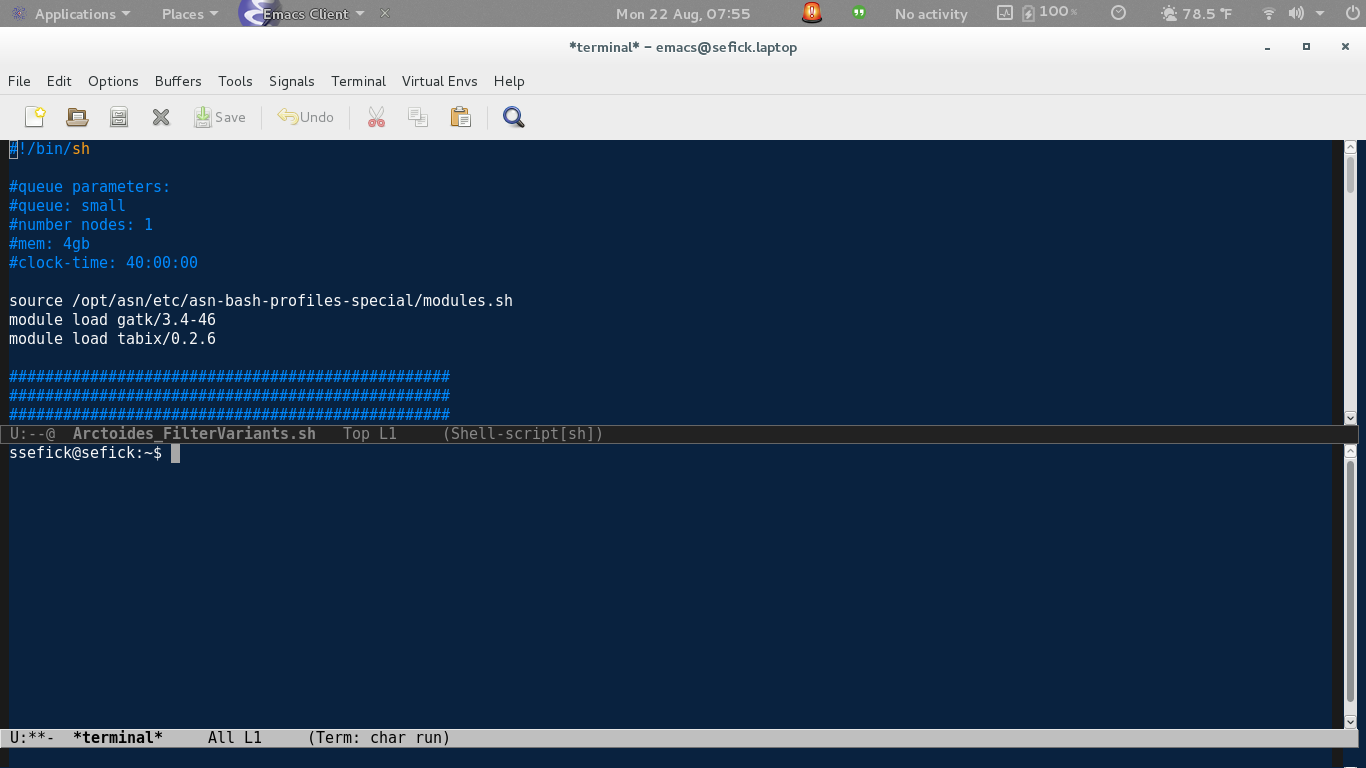
\includegraphics[width=.9\linewidth]{./sh_IDE.png}
\end{frame}
\begin{frame}
\frametitle{Emacs Speaks Statistics R (ESS)}
\label{sec-3-3}

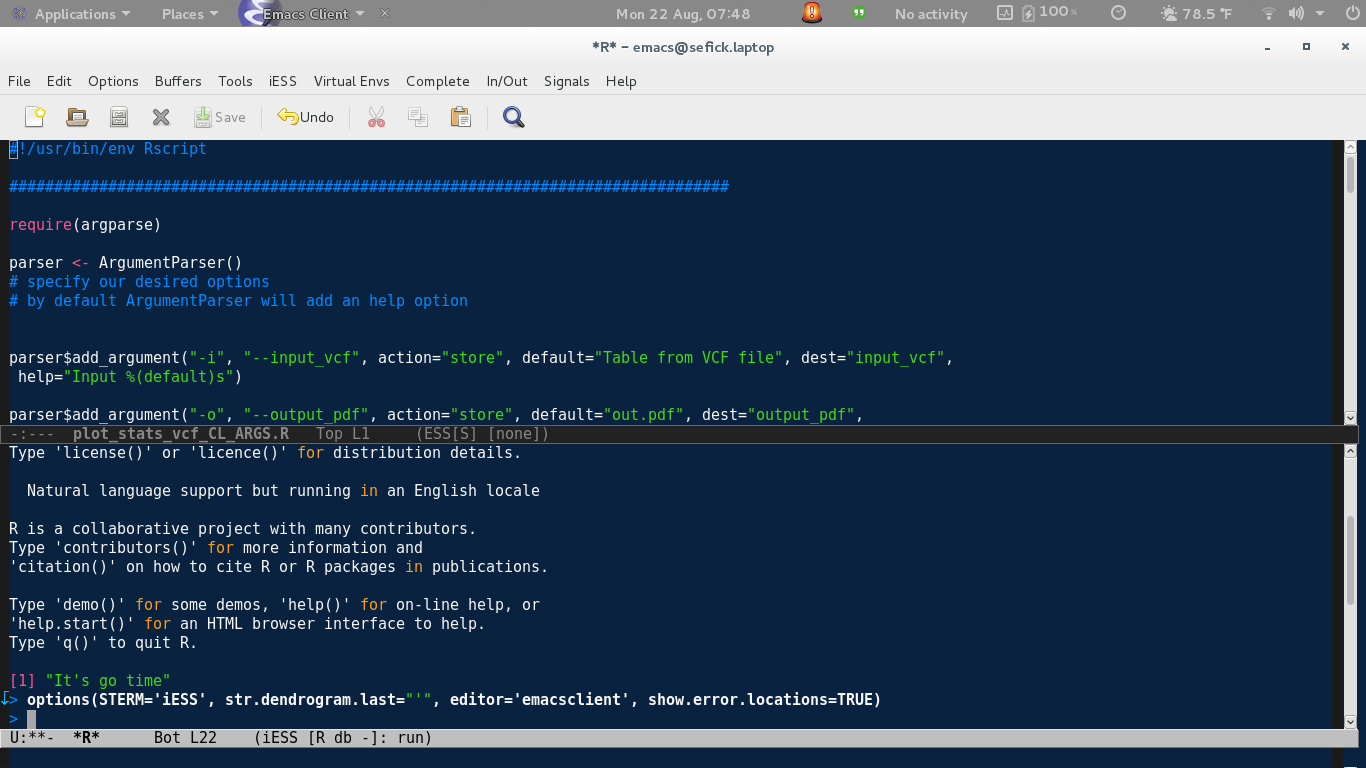
\includegraphics[width=.9\linewidth]{./ESS_IDE.png}
\end{frame}
\begin{frame}
\frametitle{Markdown: Emacs}
\label{sec-3-4}

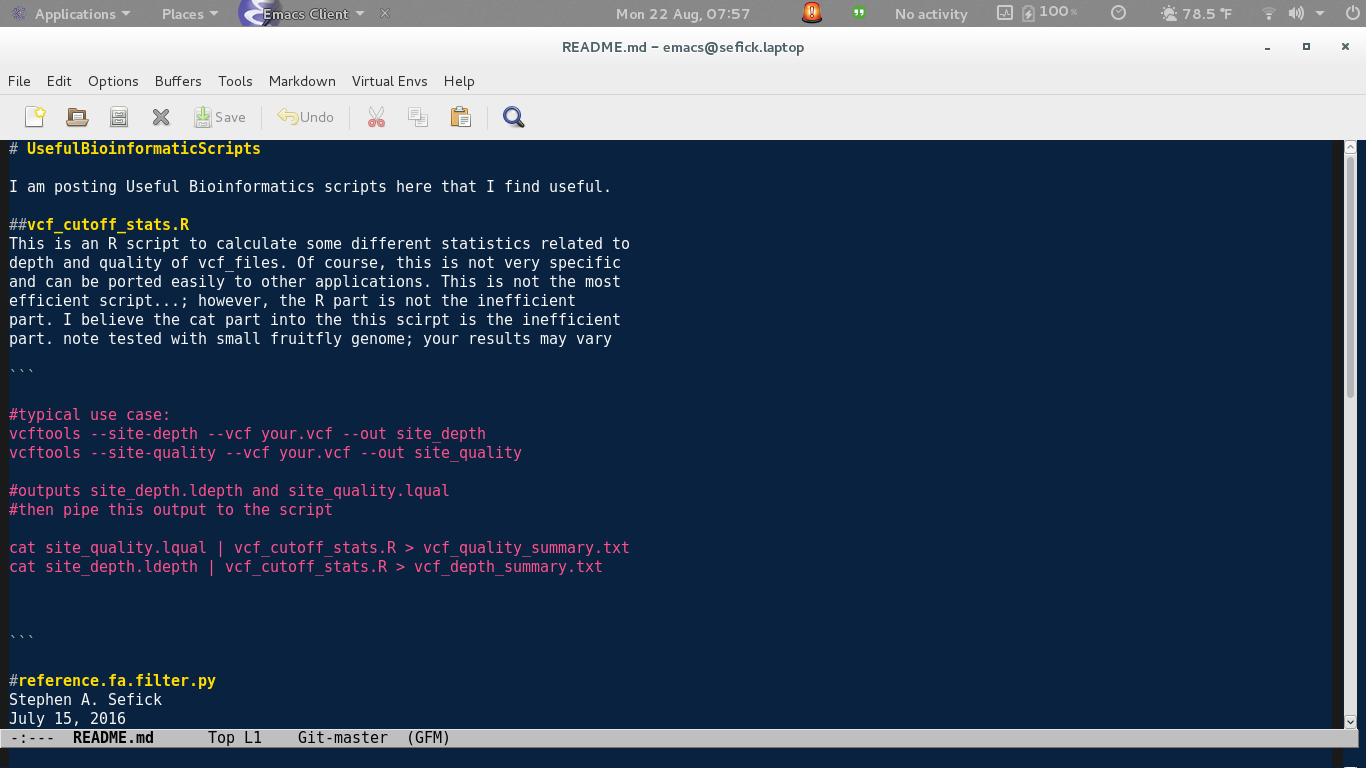
\includegraphics[width=.9\linewidth]{./README_md.png}
\end{frame}
\begin{frame}
\frametitle{Markdown: Github}
\label{sec-3-5}

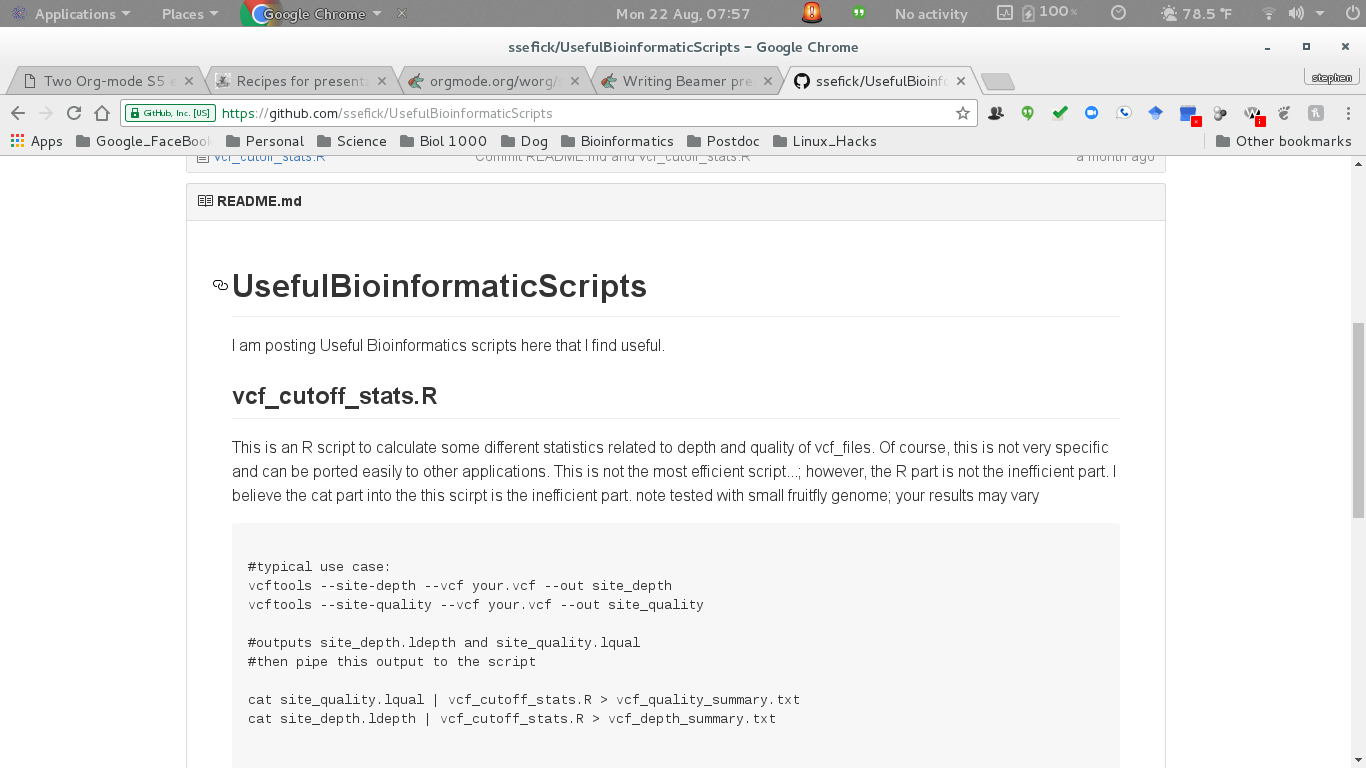
\includegraphics[width=.9\linewidth]{./README_md_GITGUB.png}
\end{frame}
\begin{frame}
\frametitle{Many others}
\label{sec-3-6}

\begin{itemize}
\item Python
\item Perl
\item C
\item Java
\item etc., etc., etc.
\end{itemize}
\end{frame}
\section{Conclusions}
\label{sec-4}
\begin{frame}
\frametitle{Text Editing Rules!}
\label{sec-4-1}

\begin{itemize}
\item 1 program/many uses
\item No loss of focus
\item More time with fingers on keyboard
\end{itemize}
\vspace{0.5}
\begin{itemize}

\item Minimal setup I would recomend
\label{sec-4-1-1}%
\begin{itemize}
\item Markdown
\item ESS
\item Python/Perl IDE
\end{itemize}

\vspace{0.5}

\item Further Help (Emacs was scary to me in June!!!)
\label{sec-4-1-2}%
\begin{itemize}
\item Google
\item \textbf{Just start EXPERIMENTING!}
\end{itemize}


\end{itemize} % ends low level
\end{frame}
\section{Exercise}
\label{sec-5}
\begin{frame}
\frametitle{Sort a bed file}
\label{sec-5-1}


\begin{itemize}
\item Bed files define genomic regions
\end{itemize}
\vspace{0.25in}
\begin{itemize}
\item sim.bed is a bedfile generated from a VCF SNP file
\end{itemize}
\vspace{0.25in}
\begin{itemize}
\item We need to sort it for downstream analysis
\end{itemize}
\vspace{0.25in}
\begin{itemize}
\item Let's write a bash script to do this
\end{itemize}
\vspace{0.25in}
\begin{itemize}
\item Things to remember about the terminal in Emacs
\begin{itemize}
\item when in charmode (default) acts like a terminal
\item when in linemode acts like an emacs buffer
\end{itemize}
\end{itemize}
\end{frame}
\begin{frame}
\frametitle{Exercise}
\label{sec-5-2}

Point play around with emacs \\ Work together \\ Do not get bogged down with \textbf{sort} command 
\vspace{0.25in}

\begin{enumerate}
\item unzip Emacs\_exercise.zip
\item open emacs in Emacs\_exercise folder
\begin{itemize}
\item emacs -nw
\end{itemize}
\item split buffer
\item move to other buffer and start terminal
\item while the focus is in the terminal change to linemode
\item Try to navigate with keyboard shortcuts
\item use ls and then copy sim.bed
\item move back to script window and paste
\item now write a script to sort the bed file
\end{enumerate}
 
\end{frame}
\section{Test Slides}
\label{sec-6}
\begin{frame}
\frametitle{What are CNTs?}
\label{sec-6-1}
\begin{columns}
\begin{column}{0.6\textwidth}
\begin{block}{when? who?}
\label{sec-6-1-1}

\begin{itemize}
\item 1952 bla bla bla
\item 1991 Dr. Sumio Iijima publishes ``Helical microtubules of graphitic carbon''
\end{itemize}
\end{block}
\end{column}
\begin{column}{0.4\textwidth}
%% Column 2
\label{sec-6-1-2}

    
\includegraphics[width=\textwidth]{./emacs5-512.png}
\end{column}
\end{columns}
\end{frame}

\end{document}
